\documentclass{scrreprt}
\usepackage{listings}
\usepackage{underscore}
\usepackage{graphicx}
\usepackage[bookmarks=true]{hyperref}
\usepackage[utf8]{inputenc}
\usepackage[english]{babel}
\hypersetup{
    bookmarks=true,    % show bookmarks bar?
    pdftitle={Software Requirement Specification},    % title
    pdfauthor={Tejaswini Durge, Arya Kadam, Chinmay Kale, Prasad Kute},                     % author
    pdfsubject={Remote MCP Control System - Autonomous LLM Admin},                        % subject of the document
    pdfkeywords={SRS, Software Requirements, MCP, LLM, Telegram}, % list of keywords
    colorlinks=true,       % false: boxed links; true: colored links
    linkcolor=blue,        % color of internal links
    citecolor=black,       % color of links to bibliography
    filecolor=black,       % color of file links
    urlcolor=blue,       % color of external links
    linktoc=page           % only page is linked
}
\def\myversion{1.0}
\date{}

\begin{document}

\begin{titlepage}
    \begin{flushright}
        \rule{16cm}{5pt}\vskip1cm
        \begin{bfseries}
            \Huge{SOFTWARE REQUIREMENTS\\ SPECIFICATION}\\
            \vspace{1.5cm}
            for\\
            \vspace{1.5cm}
            \Large{Remote MCP Control System - Autonomous System Admin}\\
            \vspace{1.5cm}
            \Large{Prepared by :}\\
            \vspace{0.5cm}
            1. Tejaswini Durge (22210270)\\
            2. Arya Kadam (22210766)\\
            3. Soham Deshmukh (22211060)\\
            4. Prasad Kute (22210330)\\
            \vspace{1.5cm}
            \Large{Submitted to :}\\
            \vspace{0.5cm}
            Prof. Hanmant Magar\\
            \vspace{1.5cm}
            \Large{\today}\\
        \end{bfseries}
    \end{flushright}
\end{titlepage}

\tableofcontents
\newpage

\chapter{Introduction}
\label{chap:introduction}

\section{Purpose}
\label{sec:purpose}
This Software Requirements Specification (SRS) document formally defines the operational, technical, and security parameters for the \textbf{Remote MCP Control System} - an innovative architecture for autonomous system administration via Large Language Models (LLMs). The document serves three primary objectives:

\begin{itemize}
    \item \textbf{System Blueprint}: Provide a complete architectural specification mapping the natural language inputs to operating system execution.
    \item \textbf{Security Assurance}: Define the strict execution sandboxing and hierarchical access permissions protecting against Arbitrary Code Execution (ACE).
    \item \textbf{Extensibility Framework}: Establish the plugin architecture guidelines utilizing Anthropic's Model Context Protocol (MCP) for future expansions.
\end{itemize}

\section{Scope}
\label{sec:scope}
The Remote MCP Control System revolutionizes direct computer administration through its multi-component architecture bridging stochastic AI reasoning with deterministic host hardware:

\subsection*{Core Features}
\begin{itemize}
    \item \textbf{Ubiquitous Interaction Layer}:
    \begin{itemize}
        \item Telegram Bridge serving as the encrypted, asynchronous mobile frontend.
        \item User session context and stateful command memory.
    \end{itemize}
    
    \item \textbf{Semantic Reasoning Engine}:
    \begin{itemize}
        \item OpenCode Agent interpreting natural language into serialized JSON-RPC tool calls.
        \item Dynamic task breakdown and procedural automation.
    \end{itemize}

    \item \textbf{Secure Execution Host}:
    \begin{itemize}
        \item FastMCP Server exposing system primitives (File I/O, Shell execution, Python evaluation).
        \item Multi-layered OS-primitive sandboxing for malicious command interception.
    \end{itemize}
\end{itemize}

\section{Definitions, Acronyms, and Abbreviations}
\label{sec:definitions}
\begin{description}
    \item[MCP] Model Context Protocol (Anthropic's open standard for AI tool integration)
    \item[LLM] Large Language Model
    \item[RCE] Remote Code Execution
    \item[ACE] Arbitrary Code Execution
    \item[AST] Abstract Syntax Tree
    \item[RPC] Remote Procedure Call (JSON-RPC 2.0)
    \item[RBAC] Role-Based Access Control
\end{description}

\section{References}
\label{sec:references}
\begin{itemize}
    \item \textbf{Project Documentation}: \url{README.md} and \url{Paper.md} \\
    \footnotesize{Primary architectural context, research methodology, and runtime specifications.}
    
    \item \textbf{Anthropic MCP Spec}: \url{https://docs.anthropic.com/en/docs/mcp/} \\
    \footnotesize{Official documentation defining the JSON-RPC integration layer used by FastMCP.}
    
    \item \textbf{Telegram Bot API}: \url{https://core.telegram.org/bots/api} \\
    \footnotesize{Transport layer documentation defining the asynchronous webhooks and client state management.}
\end{itemize}

\section{System Overview}
\label{sec:system-overview}
The Remote MCP Control System acts as a deterministic, secure gatekeeper that receives natural language from authenticated users, translates it via an LLM into explicit tool-calling schemas, and executes those commands locally within a rigidly confined sandbox.

\begin{figure}[htbp]
    \centering
    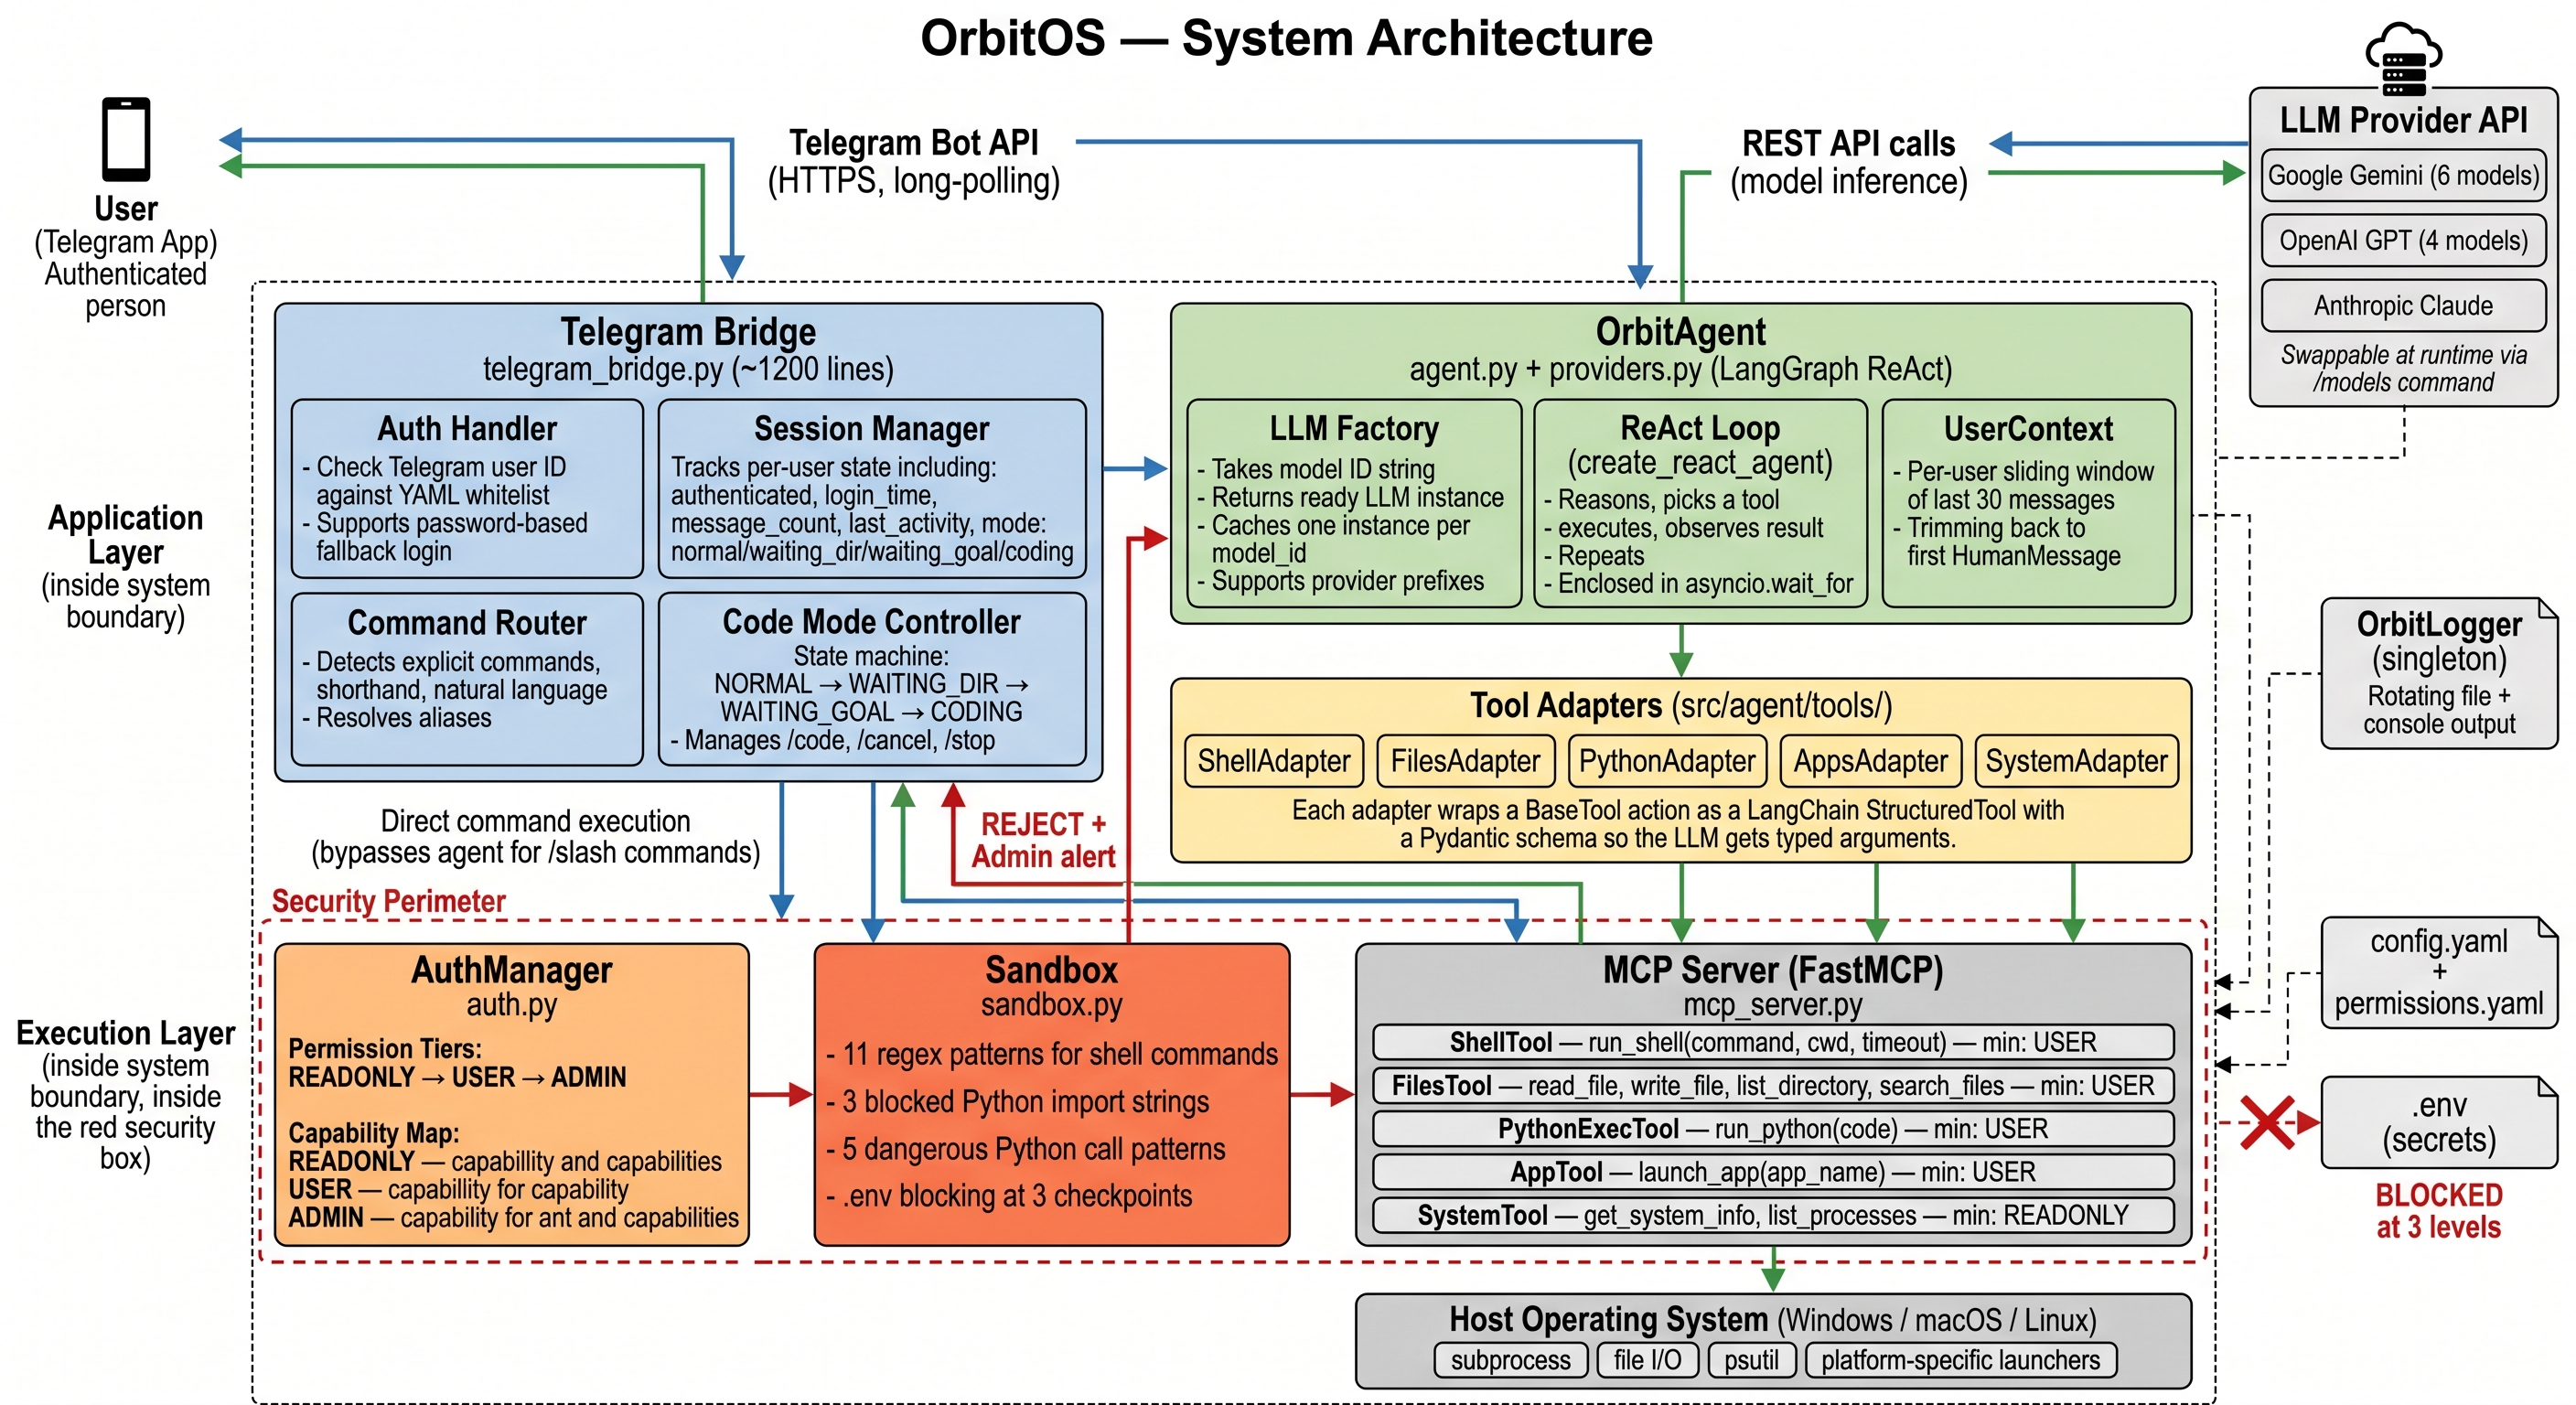
\includegraphics[width=0.92\textwidth]{system_architecture.png}
    \caption{High-Level System Architecture Diagram}
    \label{fig:system-architecture}
\end{figure}

\chapter{Overall Description}
\label{chap:overall-description}

\section{Product Perspective}
\label{sec:product-perspective}
The system employs a multi-service pipelined architecture designed to cleanly decouple user UI, LLM reasoning, and host execution:

\begin{itemize}
    \item \textbf{Frontend Layer}:
    \begin{itemize}
        \item Telegram Bot API providing interaction modalities.
        \item Context-aware session management parsing raw shortcuts vs semantic dialogue.
    \end{itemize}
    
    \item \textbf{Core Logic Layer}:
    \begin{itemize}
        \item OpenCode Agent constructing structured prompts and evaluating MCP resource availability.
        \item Context memory window tracking historical decisions.
    \end{itemize}
    
    \item \textbf{Execution / Data Layer}:
    \begin{itemize}
        \item Local FastMCP instance functioning as a resource server.
        \item Python subprocess and \texttt{exec()} modules functioning under AST-filtered namespaces.
    \end{itemize}
\end{itemize}

\section{Product Functions}
\label{sec:product-functions}

\subsection{Administrative Core}
\begin{itemize}
    \item \textbf{Dynamic Shell Operations}: Captures \texttt{stdout}/\texttt{stderr} to allow LLM agents to verify their own actions iteratively.
    \item \textbf{Intelligent File Operations}: Supports absolute/relative path resolution, file reading, and secure writing without arbitrary directory traversal vulnerabilities.
    \item \textbf{Sandboxed Python Automation}: Accepts script payloads from the LLM, filters out malicious network/OS imports via AST parsing, and executes dynamic automation locally.
\end{itemize}

\subsection{Security Management}
\begin{itemize}
    \item \textbf{Cryptographic Identity}: All connections are rejected unless authenticated against a master \texttt{permissions.yaml} utilizing hardcoded Telegram User IDs.
    \item \textbf{Granular Roles}:
    \begin{itemize}
        \item \texttt{Readonly}: Restricted to system telemetry and file consumption.
        \item \texttt{User}: Permitted to execute safe logic flows without root privileges.
        \item \texttt{Admin}: Unrestricted system modification and shell access.
    \end{itemize}
\end{itemize}

\section{User Characteristics}
\label{sec:user-characteristics}

\subsection{End User Profiles}
\begin{itemize}
    \item \textbf{System Administrators}:
    \begin{itemize}
        \item Highly technical profiling requiring rapid, mobile-friendly responses to server incidents.
        \item Heavy utilization of the \texttt{admin} permission class.
    \end{itemize}
    
    \item \textbf{General Users}:
    \begin{itemize}
        \item Users who want to automate tedious OS tasks ("Group my downloads by file type") without knowing shell scripting.
    \end{itemize}
\end{itemize}

\section{Operating Environment}
\label{sec:operating-environment}

\subsection{Host Requirements}
\begin{itemize}
    \item \textbf{Operating System}: Windows 10/11 natively supported; POSIX-compliant layers available.
    \item \textbf{Runtime}: Python 3.10+ (requires native \texttt{asyncio}).
    \item \textbf{Dependencies}: \texttt{fastmcp}, \texttt{python-telegram-bot}, \texttt{psutil}.
    \item \textbf{Network}: Must maintain an outbound secure HTTPS tunnel to Telegram's REST APIs; no inbound ports (e.g., 80/443) are required to be exposed.
\end{itemize}

\section{Design and Implementation Constraints}
\label{sec:design-constraints}

\begin{itemize}
    \item \textbf{Performance}: The system must acknowledge user interactions in under 1 second (e.g., "Thinking...") to comply with Telegram's UX latency standards.
    \item \textbf{Security}: Due to the lack of hardware virtualization (MicroVMs), safety relies heavily on blacklists and Abstract Syntax Tree (AST) scanning. Any bypass by an LLM hallucination represents a critical vulnerability.
    \item \textbf{Coupling}: The architecture strictly mandates the use of Anthropic's standard Schema specifications to ensure the system doesn't break when switching downstream LLM providers.
\end{itemize}

\chapter{Functional Requirements}

\section{Authentication and Security Enforcement}
\begin{itemize}
    \item \textbf{FR1}: The system must extract the Telegram user's ID on every incoming payload and validate it against the \texttt{config/permissions.yaml} file.
    \item \textbf{FR2}: Unregistered payloads must be silently dropped or return a generic "Unauthorized" message to prevent endpoint enumeration.
    \item \textbf{FR3}: The FastMCP server must enforce Role-Based Access Control (RBAC) prior to executing any subprocess.
\end{itemize}

\section{Agent Reasoning \& NLP}
\begin{itemize}
    \item \textbf{FR4}: The \texttt{OpenCodeAgent} must maintain a conversational memory limit (e.g., maximum 20 messages) to prevent context window exhaustion.
    \item \textbf{FR5}: The agent must parse vague natural language into explicit JSON-RPC payloads conformant to the MCP specification.
    \item \textbf{FR6}: The agent must interpret failure streams (\texttt{stderr}) from the host and attempt autonomous self-correction without immediate user intervention.
\end{itemize}

\section{Core Execution Tools}
\begin{itemize}
    \item \textbf{FR7}: The \texttt{ShellTool} must execute non-interactive commands within a maximum timeout of 30 seconds to prevent resource exhaustion (DoS).
    \item \textbf{FR8}: The \texttt{FilesTool} must restrict operations to authorized absolute directories, preventing arbitrary traversal (e.g., accessing \texttt{C:/Windows/System32} illegally).
    \item \textbf{FR9}: The \texttt{PythonExecTool} must parse execution strings utilizing Python's native \texttt{ast} module and flag node types attempting imports of \texttt{os}, \texttt{sys}, or \texttt{subprocess}.
\end{itemize}

\subsection{Use Case Diagram}
\begin{figure}[h]
    \centering
    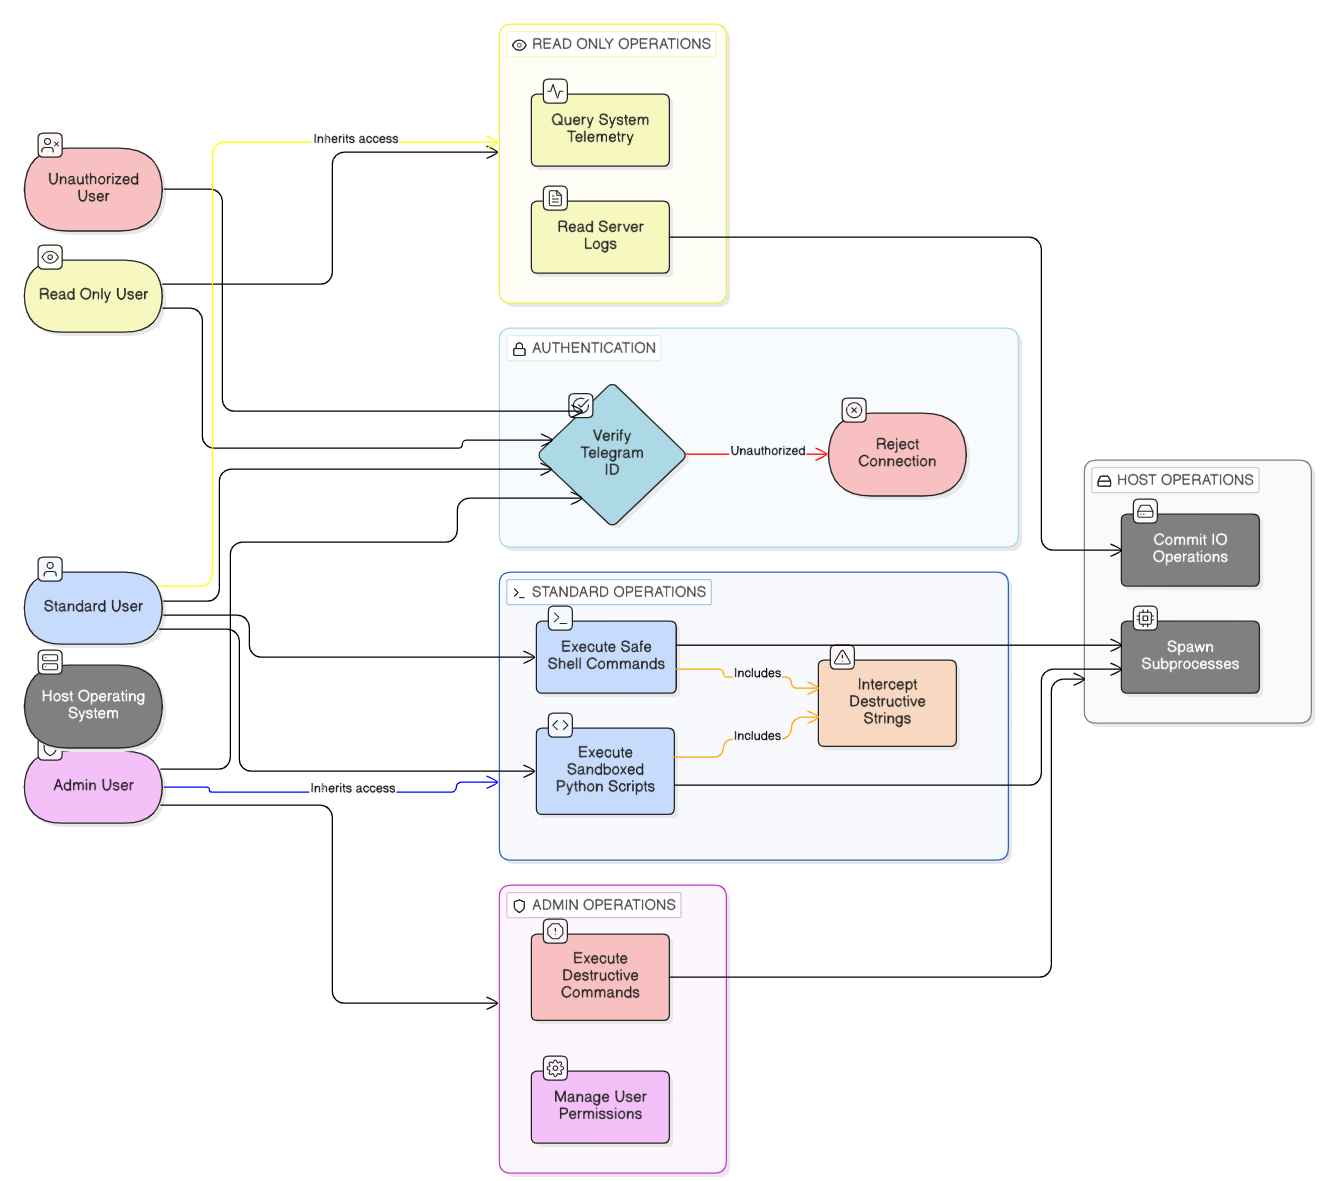
\includegraphics[width=\textwidth]{use_case_diagram.png}
    \caption{System Use Case Diagram}
    \label{fig:use_case_diagram}
\end{figure}

\chapter{Non-Functional Requirements}

\section{Security}
\begin{itemize}
    \item \textbf{NFR1}: The Telegram API Token and local authentication passwords must never be logged or hardcoded, residing exclusively in \texttt{.env} dotfiles.
    \item \textbf{NFR2}: The Sandbox primitive must evaluate destructive shell commands prior to thread instantiation; failure to catch a destructive string must result in system soft-lock rather than execution sequence continuation.
\end{itemize}

\section{Performance}
\begin{itemize}
    \item \textbf{NFR3}: Direct deterministic tool calls routing around the LLM agent (e.g., \texttt{/shell ping 8.8.8.8}) must execute and return to the UI in less than 800 milliseconds.
    \item \textbf{NFR4}: The FastMCP server process threading must not consume more than 2\% of idle CPU state.
\end{itemize}

\section{Usability \& Maintainability}
\begin{itemize}
    \item \textbf{NFR5}: The system architecture must allow developers to drag-and-drop new subclasses into the \texttt{plugins/} directory without modifying the central bootloops.
    \item \textbf{NFR6}: The UI must format all terminal outputs inside Telegram markdown blocks for maximal readability on mobile form factors.
\end{itemize}

\chapter{System Architecture and Interface Requirements}

\section{System Architecture}
The Remote MCP Control System effectively utilizes an event-driven Pipeline Architecture:
\begin{itemize}
    \item \textbf{Source}: User Chat Interface (Telegram Bridge routing).
    \item \textbf{Processor}: Language Model context builder (OpenCode Agent JSON-RPC framing).
    \item \textbf{Sink}: FastMCP execution server committing writes to the local Host OS.
\end{itemize}

\subsection{Data Flow Diagram}
\begin{figure}[h]
    \centering
    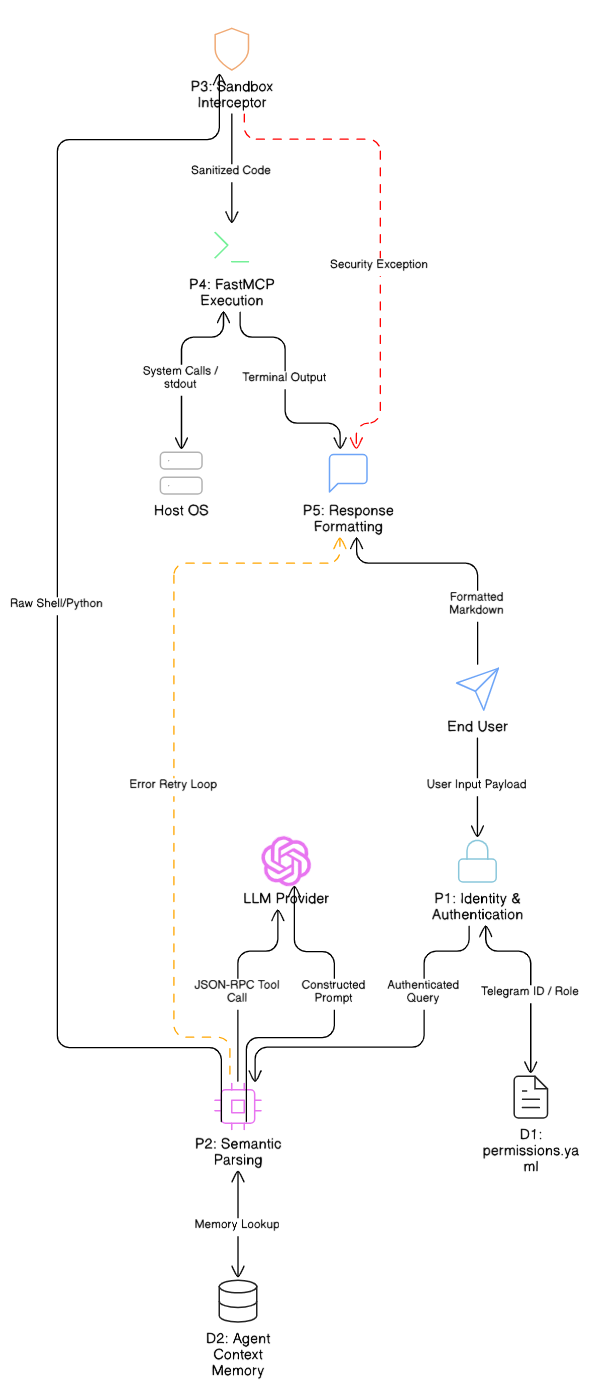
\includegraphics[width=0.75\textwidth]{data_flow_diagram.png}
    \caption{Data Flow Diagram}
    \label{fig:data_flow_diagram}
\end{figure}

\section{External Interfaces}
\subsection{Communication Interfaces}
\begin{itemize}
    \item Secure HTTPS transport bound exclusively utilized for downstream Telegram API communications.
    \item Locally bound sockets (e.g., \texttt{localhost:8765}) used for inter-process communication between the Agent Client and the MCP Server, guaranteeing the execution boundary cannot be compromised externally.
\end{itemize}

\chapter{Validation and Verification Requirements}
\section{Testing Strategy}
\begin{itemize}
    \item \textbf{Red-Team Penetration}: Simulating prompt-injection attacks directly into the OpenCode Agent to evaluate the efficacy of the \texttt{Sandbox} interceptors.
    \item \textbf{Unit Testing}: Ensuring AST parsing correctly identifies heavily obfuscated, implicitly nested import statements.
    \item \textbf{End-to-End Validation}: User testing the system with highly vague prompts to confirm the LLM reliably self-corrects based on recursive \texttt{stderr} logging.
\end{itemize}

\chapter{Appendices}
\section{Glossary}
\begin{itemize}
    \item \textbf{MCP}: Model Context Protocol.
    \item \textbf{AST}: Abstract Syntax Tree.
    \item \textbf{JSON-RPC}: A remote procedure call protocol encoded in JSON.
    \item \textbf{Sandboxing}: A security mechanism separating running programs, often used to execute untested or untrusted code locally.
\end{itemize}

\section{System Diagrams}
\label{sec:system_diagrams}

\subsection{Sequence Diagram}
\begin{figure}[h]
    \centering
    \includegraphics[width=\textwidth]{sequence_diagram.png}
    \caption{Sequence Diagram}
    \label{fig:sequence_diagram}
\end{figure}

The system architecture and workflows are visualized through the following diagrams, which provide both high-level overviews and detailed operational perspectives:

\begin{itemize}
    \item \textbf{Figure \ref{fig:system-architecture}}: High-Level System Architecture Diagram \\
    Details the isolation boundary between the Telegram API, the Agent semantic layer, and the local host operating system.

    \item \textbf{Figure \ref{fig:use_case_diagram}}: Use Case Diagram \\
    Captures user-system interactions depending strictly on the RBAC \texttt{permissions.yaml} assigned roles (ReadOnly, User, Admin).

    \item \textbf{Figure \ref{fig:data_flow_diagram}}: Data Flow Diagram \\
    Demonstrates the temporal progression of a natural language string converting into structured execution instructions via the Data and Transport layers of the MCP protocol.

    \item \textbf{Figure \ref{fig:sequence_diagram}}: Sequence Diagram \\
    Illustrates the precise operational lockstep occurring within the \texttt{Sandbox} intercept module during an attempted Arbitrary Code Execution event.
\end{itemize}

\end{document}
